\documentclass[main]{subfiles}
\begin{document}

%@@@@@@@@@@@@@@@@@@@@@@@@@@@@@@
% Main Topics: Nervous System Organization - 27.09.2018
% Lecturer: Wolfger von der Behrens
% author: Vanessa Leite - base document from benelot/eth-intro-to-neuroinformatics-summary

\section{Nervous System Organization}
\subsection{Anatomy}
\begin{itemize}[noitemsep,nolistsep]
	\item Central nervous system (CNS): Brain and spinal cord.
	\item Peripheral nervous system (PNS): somatic and autonomic (sympathetic and parasympathetic) NS.
	\subitem sympathetic NS: driven by adrenalin - fight/flight reactions
	\subitem parasympathetic NS: rest and digest
	\item Cranial nerves: they are the gates between the sensory periphery and our brain.
	\item Brain cuts: Horizontal plane cut, coronal/frontal cut and sagittal cut (between eyes). Cross-section through spinal cord, for example.
	\item The skull protects, meninges envelope the CNS and has 3 layers, the dura mater, arachnoid mater and pia mater. Primary function is protection.
	\item The cortex is the layer directly under the surface of the brain.
	\item There are 4 lobes in each hemisphere. Lobes are separated by fissures in the cortex.
\end{itemize}

\subsubsection{The human brain}
\begin{itemize}
\item Volume of human brain started to increase 2 million years ago
\item Most of the studies do not use human brain, they use mouse brain (70 million neurons) instead.
\end{itemize}

\subsubsection{Gross anatomy of the brain}
\begin{itemize}
\item Skull has 32 bones, its main function is to protect the brain. The hardest bone in the body is the skull.
\item The skull provides fixed points for senses (eyes, ears, etc.)
\item Below the skull we find the meninges, they protect the brain against infections
\subitem dura mater
\subitem arachnoid mater
\subitem pia mater: follows the brain surface/curvature
\item The brain has 4 cavities filled with Cerebral Spinal Fluid (CSF). This is as a protection so the brain do not touch the bones and do not damage itself.
\item To "navigate" the brain we use coronal, saggital and horizontal planes.
\subitem coronal plane: divides the brain in anterior (rostral) and posterior (caudal) parts.
\subitem saggital plane: divides the brain in left/right parts.
\subitem horizontal plane: divides the brain in superior/inferior parts.
\end{itemize}

\subsubsection{Building elements of the brain}
The brain develops from the neural plate.

\begin{itemize}[noitemsep,nolistsep]
	\item Forebrain (Prosencephalon): Cortex, thalamus, hippocampus, basal ganglia, corpus callosum.
	\item Midbrain (Mesencephalon): Tectum, tegmentum.
	\item Hindbrain (Rhombencephalon): Cerebellum, pons, medulla oblongata.
	\item White matter: Glia cells, myelinated axons.
	\item Grey matter: Neurons (soma).
	\item Neocortex: Six-layered cortex that forms the surface of most of the cerebral hemispheres.
	\item Corpus callosum: Midline fiber bundle, connects the two cerebral hemispheres.
	\item Gyrus: Ridges of the cotex, with valleys (sulci).
\end{itemize}

\begin{figure}[H]
	\centering
	\begin{subfigure}[b]{0.5\textwidth}
		\centering
		\includegraphics[width=\textwidth]{brain-parts.png}
	\end{subfigure}%
	~
	\begin{subfigure}[b]{0.5\textwidth}
		\centering
		\includegraphics[width=\textwidth]{brain.png}
	\end{subfigure}
\end{figure}
\begin{figure}[H]
	\centering
	\includegraphics[width=\textwidth]{brain_anatomy_01.png}
\end{figure}
\begin{figure}[H]
	\centering
	\begin{subfigure}[b]{0.5\textwidth}
		\centering
		\includegraphics[width=\textwidth]{motor-sensory-neuron.png}
	\end{subfigure}%
	~
	\begin{subfigure}[b]{0.5\textwidth}
		\centering
		\includegraphics[width=\textwidth]{brain-cut.png}
	\end{subfigure}
\end{figure}

\subsubsection{The limbic system}
It is related with our emotions.

\begin{itemize}[noitemsep,nolistsep]
	\item Structure: On medial and basal surfaces of cerebral hemispheres.
	\item Includes cingulate gyrus, parahippocampal gyrus, hippocampal formation, fornix, amygdala, septum, mamillary bodies
	\item Function: Emotional expression, memory acquisition, fear conditioning, violence and aggression.
	\item amygdala is really important for fear condition.
\end{itemize}
\begin{figure}[H]
	\centering
	\begin{subfigure}[b]{0.5\textwidth}
		\centering
		\includegraphics[width=\textwidth]{brain_anatomy_02.png}
	\end{subfigure}%
	~
	\begin{subfigure}[b]{0.5\textwidth}
		\centering
		\includegraphics[width=\textwidth]{brain_anatomy_03.png}
	\end{subfigure}
\end{figure}

\subsubsection{Hypothalamus and thalamus}
Thalamus is the "gate to the cortex"

\begin{itemize}[noitemsep,nolistsep]
	\item The thalamus structure is relatively large with two symmetric large nuclei (receiving ascending and descending inputs) and many projections.
	\item Thalamus function: relay station, domain-specific information processing.
	\item The upper brain stem is the diencephalon.
	\item The hypothalamus is very small and controls autonomic mechanisms.
	\item Pituitary gland: controls hunger, body temperature, etc.
\end{itemize}

\subsubsection{Basal ganglia}
It is related with movement control. It triggers the movement, not the fine movement control. It is formed by caudate nucleus + putamen + globus pallidus +
substantia nigra + subthalamic nucleus.

\begin{itemize}[noitemsep,nolistsep]
	\item Structure: Collection of nuclei embedded deep within the cortex.
	\item Partially surrounds the thalamus.
	\item Sensory projectons to the cerebrum
	\item Function: Regulate voluntary movement.
	\item Movement disorders like Parkinson's.
\end{itemize}

\subsubsection{Cerebellum}
\begin{itemize}[noitemsep,nolistsep]
	\item Structure: ``little brain'', has layered appearance and symmetry.
	\item Two hemispheres are connected by the vermis.
	\item Function: Coordinated motor behavior, posture adjustments and stores memories for simple learned motor responses.
\end{itemize}

\subsubsection{Reticular Formation}
\begin{itemize}[noitemsep,nolistsep]
	\item Structure: Diffuse arrangement of ascending and descending neurons.
	\item Function: Arousal, selective attention, respiration.
\end{itemize}

\subsubsection{Cortical areas}
\begin{itemize}
\item Phineas Gage: accident in 1848 destroyed left frontal lobe. "The equilibrium or balance, so to speak, between his intellectual faculties and animal propensities, seems to have been destroyed".
\end{itemize}
\subsubsection{Connections}
\begin{itemize}[noitemsep,nolistsep]
	\item The Basal ganglia projects to the cerebral cortex (via thalamus).
	\item The cerebellum projects to the cerebral cortex (via thalamus).
	\item The cerebral cortex projects to basal ganglia, cerebellum and motor neurons (and interneurons) via pons.
	\item The cortex has six layers.
	\item From superficial layers to deep layers we say that we have a feedfoward connection.	From deep to superficial layers we have a feedback connection.
	
\end{itemize}

\begin{figure}[H]
	\centering
	\begin{subfigure}[b]{0.5\textwidth}
		\centering
		\includegraphics[width=\textwidth]{brain_anatomy_04.png}
	\end{subfigure}%
	~
	\begin{subfigure}[b]{0.5\textwidth}
		\centering
		\includegraphics[width=\textwidth]{brain_anatomy_05.png}
	\end{subfigure}
\end{figure}

\subsubsection{Nervous system in numbers}
\begin{itemize}[noitemsep,nolistsep]
	\item $1\,mm^3$ of white matter is $9\,m$ of axons.
	\item $1\,mm^3$ of grey matter is $50'000$ neurons.
	\item In $1\,mm^3$ about $100'000$ cells.
\end{itemize}

\subsection{Basic structure of the neuron}

\begin{figure}[H]
	\centering
	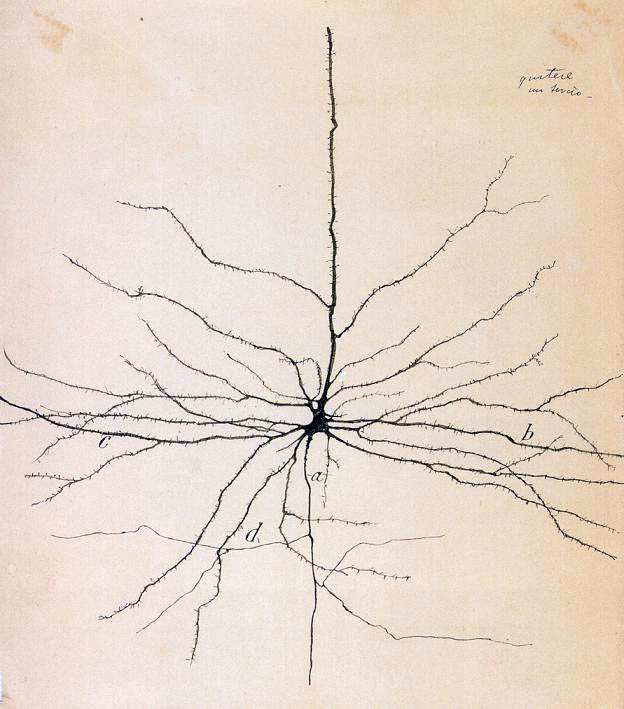
\includegraphics[width=0.5\textwidth]{pyramidal-neuron.jpg}
	\caption{Pyramidal neuron drawn by Ramon y Cajal, founder of modern neuroscience}
\end{figure}

\subsubsection{Types of neurons}
There are different types of neurons, for instance: bipolar cells, ganglion cells (retina), cortical pyramidal cells, cerebellar purkinje cells, etc. But all of them follow the same basic structure: cell body, axon and axon terminal.

\subsubsection{Components/Terminology}
\begin{itemize}[noitemsep,nolistsep]
	\item Cell body
	\item Nucleus
	\item Dendrite: input component.
	\item Axon: output component, makes contact to other neurons.
	\item Myelin: wraps around axons, makes white matter white.
	\item Boutons: at the ends of the axons, connects neurons.
	\item Soma: body of a cell without it's extensions.
	\item Afferent: neurons that carry nerve impulses from receptors to the CNS.
	\item Efferent: neurons that carry information away from the CNS.
	\item Projection neuron: neuron with long axons that project to distant targets.
\end{itemize}

\subsubsection{Axon transport}
\begin{itemize}[noitemsep,nolistsep]
	\item Golgi apparatus sits at the cell body.
	\item Transport of vesicles to the axon terminal (anterograde).
	\item Transport of empty vesicles back to the cell body (retrograde).
\end{itemize}

\subsubsection{Synapse}
Conversion between electrical to chemical signals take place in the synapse. Basic sequence: neurotransmitter release $\rightarrow$ receptor binding $\rightarrow$ ion channels open or close $\rightarrow$ conductance change causes current flow $\rightarrow$ postynaptic potential changes $\rightarrow$ postsynaptic cells excited or inhibited $\rightarrow$ summation determines whether or not an action potential occurs.

Lot of computation occurs in the synapse.

In myelinated axons we have "jumps" of action potential.

Flow of negative/positive charged ions into the neuron can lead to depolarization (excitation) or polarization (depression).

\begin{itemize}[noitemsep,nolistsep]
	\item Boutons: connection point.
	\item Cleft: little gap between presynaptic and postsynaptic neuron.
	\item Dendritic spines: dendritic part of the synapse.
	\item Transmitter: gets released by the presynaptic neuron, in vesicles.
	\item Vesicles: transport the transmitter inside the cell.
	\item Receptors: binding site for the transmitter.
	\item Postsynaptic membrane
\end{itemize}

\subsubsection{Post synaptic receptors}
\begin{itemize}
\item ligand-gated ion channels
\item g-protein-coupled receptors
\end{itemize}

\subsubsection{Networks}
A neuron receives input from many different neurons and can send information to many different neurons as well (colateral on axon).

\subsection{Muscle reflex and antagonistis}\footnote{This was not covered in 2018}
\subsubsection{Reciprocal innervation of antagonistic muscles}
\begin{enumerate}[noitemsep,nolistsep]
	\item A tack produces a burst of firing (sensory neurons, for example on the finger).
	\item The burst excites excitatory spinal interneurons, which then excite the motor neurons of a muscle.
	\item The burst also excites inhibitory spinal interneurons that inhibit antagonist muscle motor neurons.
	\item One muscle gets contracted, the other relaxed, allowing for a rapid flexion. No brain involved (but gets informed).
\end{enumerate}
\subsubsection{Elicitation of a stretch reflex}
\begin{itemize}[noitemsep,nolistsep]
	\item When hitting the knee tendon with a hammer, the spindles of the thigh muscle get stretched and this elicits a burst of firing in the spindle afferents.
	\item The burst triggers a burst of firing in the thigh muscle motor neurons, causing contraction.
\end{itemize}



\end{document}
